\documentclass{beamer}
\mode<presentation>
\usepackage{amsmath,amssymb,mathtools}
\usepackage{textcomp}
\usepackage{gensymb}
\usepackage{adjustbox}
\usepackage{subcaption}
\usepackage{enumitem}
\usepackage{multicol}
\usepackage{listings}
\usepackage{url}
\usepackage{graphicx}
\def\UrlBreaks{\do/\do-}

\usetheme{Boadilla}
\usecolortheme{lily}
\setbeamertemplate{footline}{
\leavevmode
\hbox{
\begin{beamercolorbox}[wd=\paperwidth,ht=2ex,dp=1ex,right]{author in head/foot}
\insertframenumber{} / \inserttotalframenumber\hspace*{2ex}
\end{beamercolorbox}}
\vskip0pt
}
\setbeamertemplate{navigation symbols}{}

\lstset{
frame=single,
breaklines=true,
columns=fullflexible,
basicstyle=\ttfamily\tiny
}

\numberwithin{equation}{section}

\newcommand{\myvec}[1]{\ensuremath{\begin{pmatrix}#1\end{pmatrix}}}
\let\vec\mathbf

\title{Matgeo Presentation - Problem 4.7.45}
\author{Revanth Siva Kumar.D -- EE25BTECH11048}

\begin{document}

\begin{frame}
\titlepage
\end{frame}

\begin{frame}{QUESTION}
The equation of the line passing through the point $(1, 2)$ and perpendicular to the line $x + y + 1 = 0$ is\end{frame}

\begin{frame}{Solution:}
Let desired line :
\begin{align}
    \vec{n}^T\vec{x}=c
    \label{eq:question}
\end{align}
Given line equation and point say A:
\begin{align}
    x+y+1=0
    \label{eq:line}\\
    y=-x-1\\
    \vec{A}=\myvec{1\\2}
\end{align}
Since, the line from eq \eqref{eq:line} is perpendicular to \eqref{eq:question} \\
We get the normal vector which is equal to:
\begin{align}
   \vec{n} =\myvec{1\\-1}
\end{align}

Because line \eqref{eq:line} is perpendicular, the equation of the line can be changed as:
\begin{align}
    \vec{n}^T\myvec{\vec{x} - \vec{A}}=0
\end{align}
\end{frame}
\begin{frame}{Solution:}
Thus the equation of line:

\begin{align}
    \myvec{1&-1}\myvec{\vec{x} - \myvec{1\\2}}=0\\
    \implies  \myvec{1&-1}\vec{x}-\myvec{1&-1}\myvec{1\\2}=0\\
    \implies \myvec{1&-1}\vec{x}=-1
\end{align}

\textbf{Final Answer}
The desired line equation is as follows
\begin{align*}
    \myvec{1&-1}\vec{x}=-1
\end{align*}
\end{frame}
\begin{frame}[fragile]{C Source Code: points.c}
\begin{lstlisting}[language=C]
#include <stdio.h>

// Compute slope of required line
double compute_slope() {
    // Given line: x + y + 1 = 0 → slope = -1
    double slope_given = -1.0;

    // Required line ⟂ given line → slope = -1 / slope_given
    double slope_required = -1.0 / slope_given;

    return slope_required;  // should be 1.0
}

\end{lstlisting}
\end{frame}

\begin{frame}[fragile]{Python Script: call c.py}
\begin{lstlisting}[language=Python]
import ctypes
import numpy as np

# Load shared library
lib = ctypes.CDLL("./points.so")

# Prepare array for slopes
slopes = (ctypes.c_double * 2)()
lib.compute_slopes(slopes)

slope_given = slopes[0]
slope_perp = slopes[1]

# Known point
x0, y0 = 1, 2

# Equation form: y = mx + c
def line_eqn(m, x0, y0):
    c = y0 - m * x0
    return m, c

m1, c1 = line_eqn(slope_given, x0, y0)
m2, c2 = line_eqn(slope_perp, x0, y0)

print("Given line:        y =", m1, "x +", c1)
print("Perpendicular line: y =", m2, "x +", c2)

\end{lstlisting}
\end{frame}

\begin{frame}[fragile]{Python Script: plot.py}
\begin{lstlisting}[language=Python]
import numpy as np
import matplotlib.pyplot as plt

# Given line: x + y + 1 = 0
# Perpendicular line through (1,2): slope = 1 => equation: x - y + 1 = 0

# Define range for x
x = np.linspace(-5, 5, 400)

# Equations of lines
y_given = -x - 1          # x + y + 1 = 0
y_perp  = x + 1           # x - y + 1 = 0

# Plot given line
plt.plot(x, y_given, 'b', label="Given line: x + y + 1 = 0")

# Plot perpendicular line
plt.plot(x, y_perp, 'r', label="Perpendicular line: x - y + 1 = 0")
# Plot the point (1,2)
plt.scatter(1, 2, color='k', zorder=5)
plt.text(1.1, 2.1, "(1,2)", fontsize=10)
# Add axes
plt.axhline(0, color='gray', linewidth=0.8)
plt.axvline(0, color='gray', linewidth=0.8)
# Title and labels
plt.title("Line and its Perpendicular through (1,2)")
plt.xlabel("x-axis")
plt.ylabel("y-axis")
plt.legend()
plt.grid(True)
plt.axis('equal')
plt.show()

\end{lstlisting}
\end{frame}

\begin{frame}{Result Plot}
\begin{figure}[H]
\centering
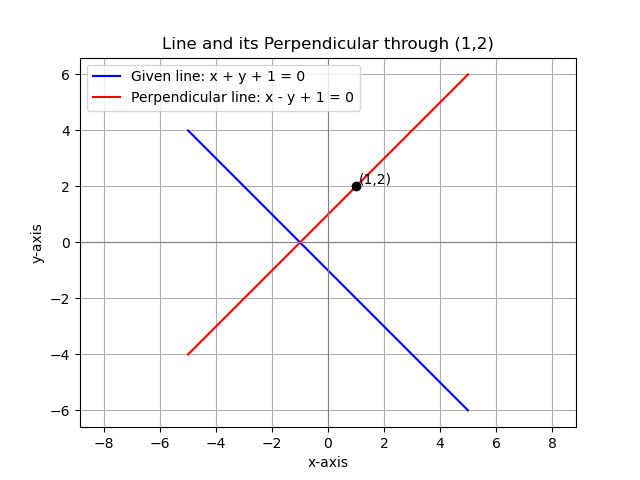
\includegraphics[width=0.7\columnwidth]{figs/Figure_1.png}
\caption*{Triangle $ABC$ plotted using shared output}
\end{figure}
\end{frame}
\end{document}











